\documentclass[]{article}
\usepackage[utf8]{inputenc}
\usepackage{xcolor}   % for textcolor
\usepackage{titlesec} % more layers of section numbering
\usepackage{geometry} % margins
\usepackage{hyperref} % references to sections
\usepackage{graphicx} % graphics path

\geometry{margin=3cm}       				   % margins
\setcounter{secnumdepth}{4} 				   % 4 layers of section numbering
\renewcommand{\thefootnote}{\arabic{footnote}} % numbered footnotes
\graphicspath{{figures/}}

\newcommand{\iso}[2]{\textsuperscript{#2}#1}   % Shortcut for isotopes


\title{Simulation and Reconstruction of Charged Particle Trajectories in~an~Atypic\footnote{\textcolor{red}{Should we change this to OFTPC as it is in the article?}} Time Projection Chamber}
\author{Martin Vavřík}
\date{June 2022}

\begin{document}
	
	\maketitle
	%\tableofcontents
	
	\section{Introduction}
		Time Projection Chamber~(TPC) is a~type of gaseous detector that detects charged particle trajectories by measuring the~position and drift time of ions created in the~gas (for more details see section~\ref{sec:tpc}). The~energy of such particles can be determined thanks to the~curvature of their trajectory in the~magnetic field.
				
		The~goal of this thesis is to develop an~algorithm for reconstruction of charged particle trajectory and energy in an~atypic TPC (with orthogonal electric and magnetic fields, abbreviation OFTPC) used in the~X17 project in IEAP~CTU\footnote{Institute of Experimental and Applied Physics, Czech Technical University in Prague}. Furthermore, we present the~results of testing this algorithm with different samples of simulated data. In future, we also wish to test this algorithm by measuring real particles with known energy distribution. In order to achieve this, we use the~Garfield++ toolkit~\cite{Garfield++} in combination with the~ROOT~framework~\cite{ROOT}. We run some of our more demanding simulations on MetaCentrum.
		
		The~X17 project in IEAP~CTU aims to replicate measurements of anomalous behavior in the distribution of angular correlation of pairs produced by the~Internal Pair Formation~(IPF) mechanism during the~decay of certain excited nuclei (\iso{Be}{8},~\iso{C}{12}~and~\iso{He}{4}) observed by the~ATOMKI group in Hungary. 
		
		\textcolor{red}{Add citations MetaCentrum, X17 project, VdG, ATOMKI papers. Maybe also TPC, IPF, ...}
		
		\subsection{ATOMKI Measurements}
			\textcolor{red}{Short summary of results of measurements in ATOMKI.}
			
		\subsection{X17 IEAP CTU}
		\label{sec:IEAP}
			\textcolor{red}{Short description of our detector. Why we use atypic TPC. Magnetic field simulations in Maxwell. Description of the coordinate system used in this thesis (+ figure).}
					
			\begin{figure}
				\centering
				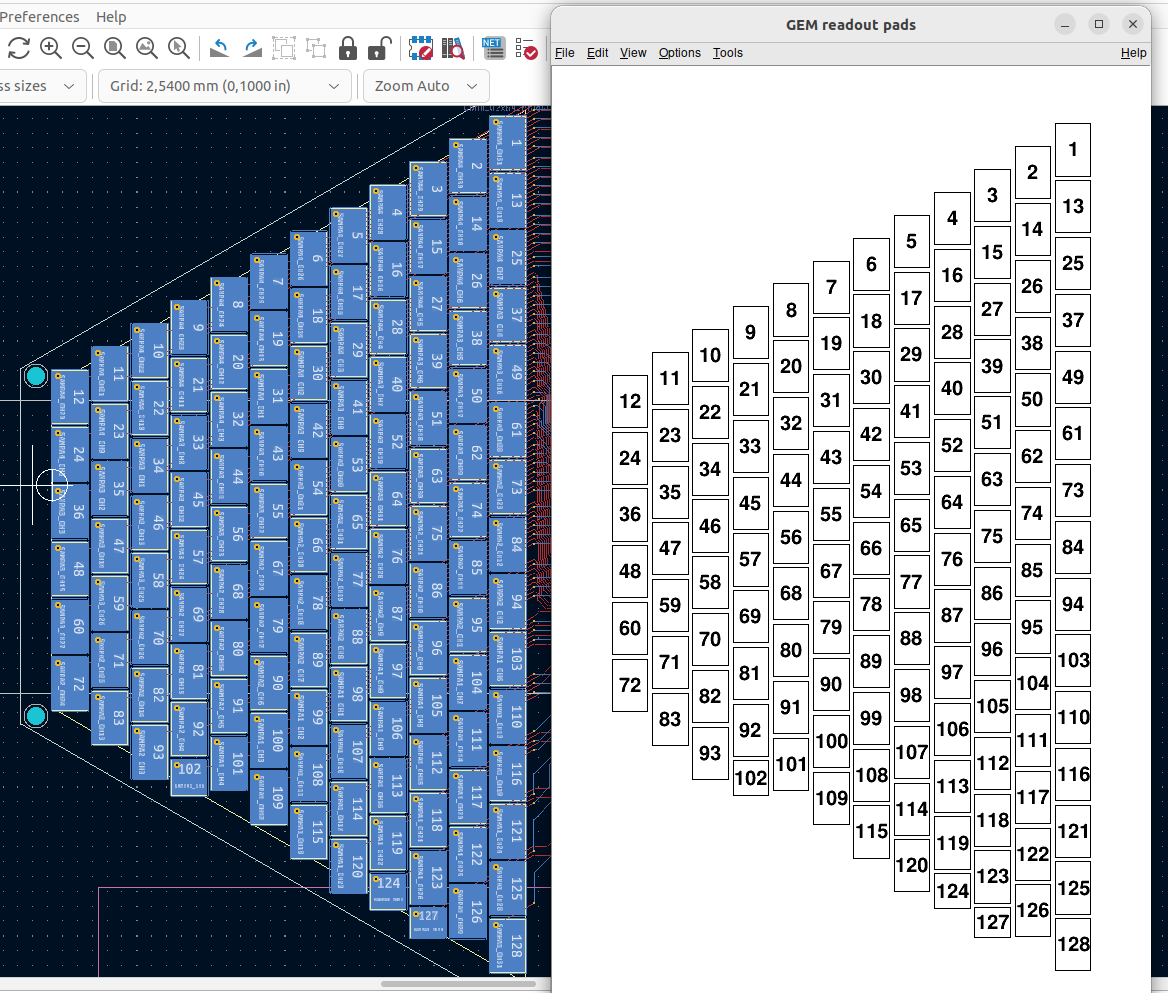
\includegraphics[width=0.8\textwidth]{padlayout.png}
				\caption{Pad layout of the TPC. \textcolor{red}{Swap for better image.}}
				\label{fig:padlayout}
			\end{figure}
	
	\section{Time Projection Chamber}
	\label{sec:tpc}
		\textcolor{red}{Description of TPC, working principle, standard vs our field layout.}
		
	\section{Track Simulation}
		In order to develop and test the~reconstruction algorithm, we simulate electron and positron tracks inside our detector with different initial parameters. We use three approaches to simulate tracks for different purposes.
		
		The \textbf{Microscopic Simulation} uses the~Garfield++ toolkit~\cite{Garfield++}. Within this toolkit, we use the~program HEED (High Energy Electro-Dynamics)~\cite{HEED} to simulate the~primary particle and class \textit{AvalancheMicroscopic} to simulate the~drift of secondary electrons created by ionization in the gas. This is the most precise and time-consuming simulation we use, our current goal is to be able to successfully reconstruct its results and determine our best case energy resolution.
		
		The \textbf{Runge-Kutta Simulation} uses the 4th order Runge-Kutta numerical integration (\textcolor{red}{add citation for Runge-Kutta}) to simulate the~trajectory of the~primary particle in the~electromagnetic field inside the~detector. It is relatively fast since it does not simulate the secondary particles. We use it as a~part of our reconstruction algorithm as well as for testing of some parts of the reconstruction.
		
		The \textbf{Fast Simulation with Ionization Electron Map} is planned for the future, it will use the~HEED program~\cite{HEED} to simulate the~primary particle and the~Ionization Electron Map (see section~\ref{sec:map}) to simulate the~drift of secondary electrons. It should be significantly faster then the~Microscopic Simulation but offer comparable precision since it will rely on already simulated drift map.
		
		All of these simulations require the~knowledge of the~electromagnetic field inside the~detector. We assume uniform electric field 400~V$\cdot$cm$^{-1}$. The~magnetic field was simulated in Maxwell (\textcolor{red}{add citation? details? own subsection with figures? more details in section~\ref{sec:IEAP}?}) by Hugo Natal da Luz.
	
		\textcolor{red}{Single track in positive x direction or initial parameters randomization.}
	
		\subsection{Microscopic Simulation}
			\textcolor{red}{Primary track simulated in HEED. Ionization electron drift simulated with AvalancheMicroscopic in Garfield.}
			
			\begin{figure}
				\centering
				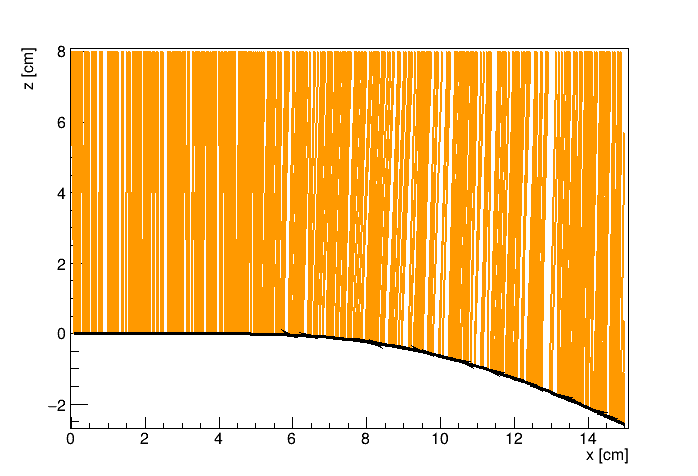
\includegraphics[width=0.3\textwidth]{7030_xz.png}
				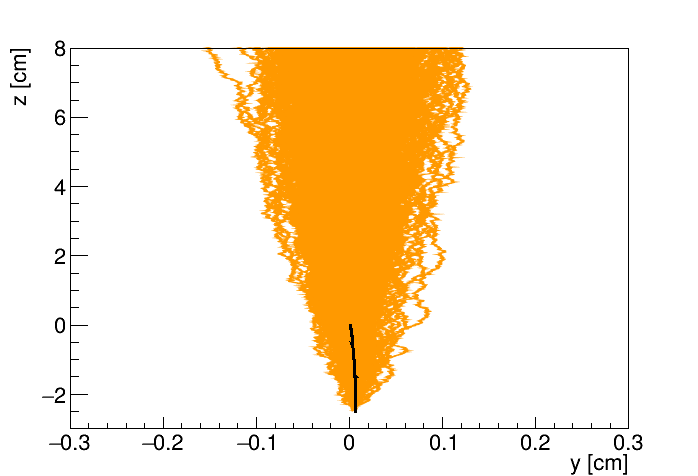
\includegraphics[width=0.3\textwidth]{7030_yz.png}
				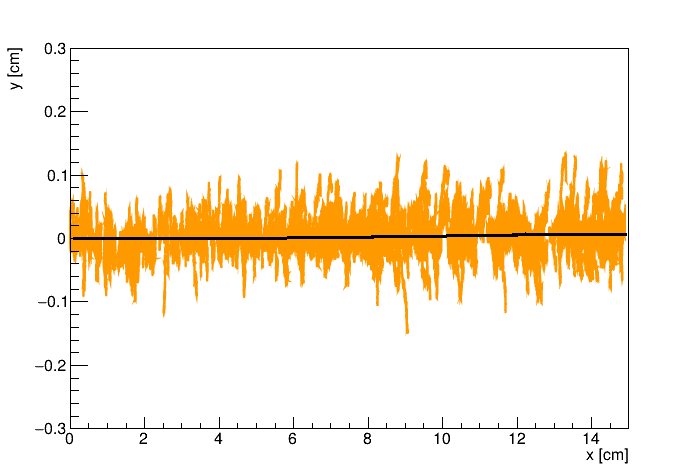
\includegraphics[width=0.3\textwidth]{7030_xy.png}
				\caption{Example of a~simulated electron track in 70~\%~argon and 30~\%~CO$_2$ atmosphere (on the left). \textcolor{red}{Swap for better images, better zoom.}}
				\label{fig:7030sim}
			\end{figure}
			
			\begin{figure}
				\centering
				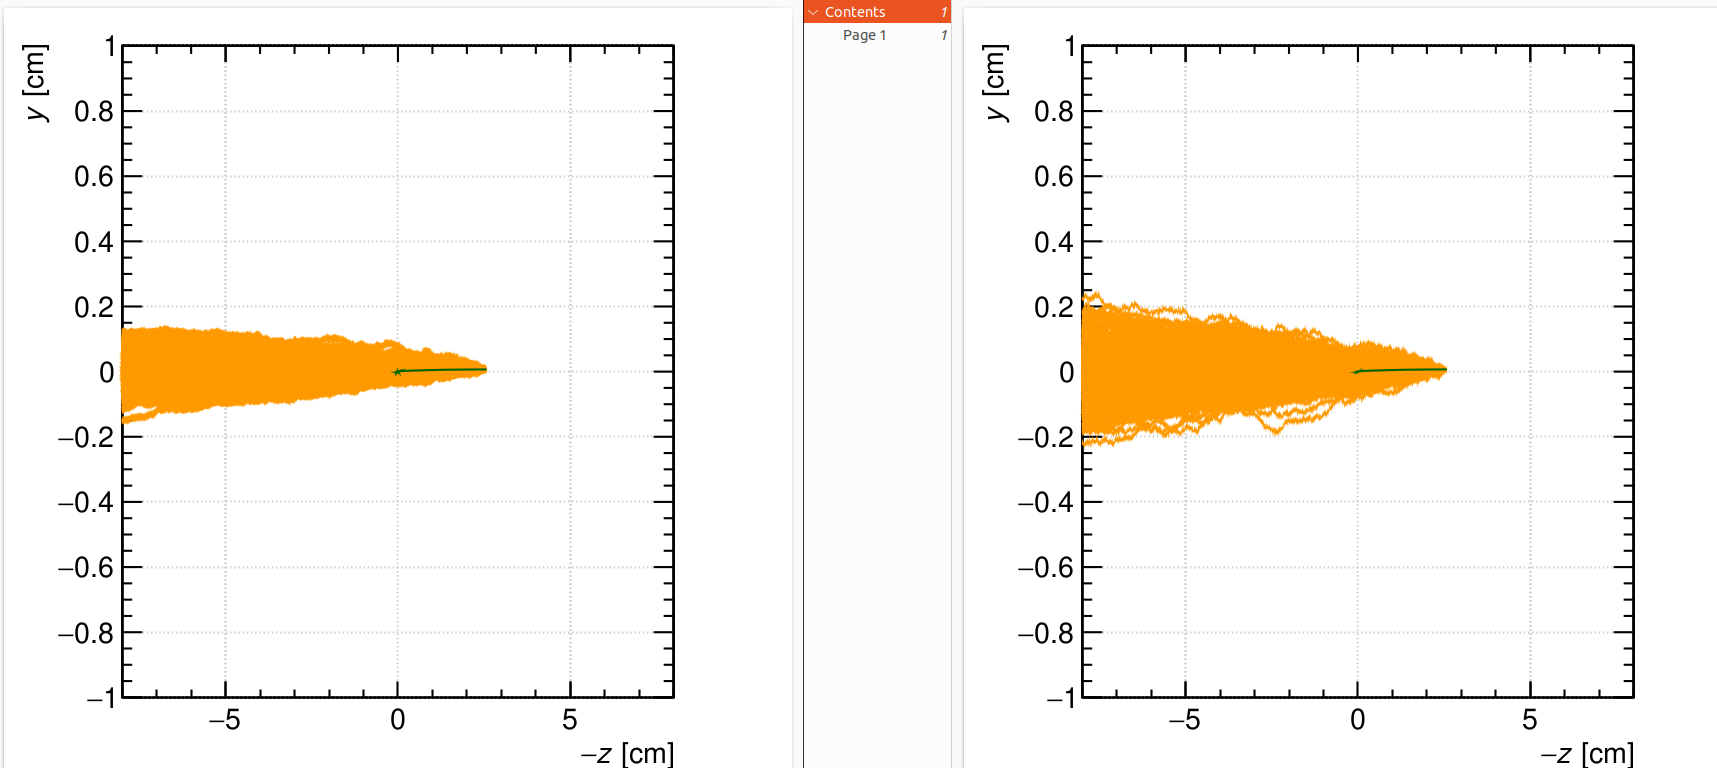
\includegraphics[width=0.9\textwidth]{diff_comp.png}
				\caption{Comparison of diffusion in a~simulated electron track in 70~\%~argon, 30~\%~CO$_2$ atmosphere and in 90~\%~argon, 10~\%~CO$_2$ atmosphere (on the right). \textcolor{red}{Swap for better image, better zoom. Or put same pictures for both comparisons in one subfigure, etc.}}
				\label{fig:diffcomp}
			\end{figure}
			
		\subsection{Runge-Kutta Simulation}
		\label{sec:rks}
			\textcolor{red}{Trajectory simulation with 4th order Runge-Kutta. Relativistic equation that is numerically integrated by the algorithm.}
			
		\subsection{Future?: Fast Simulation with the Ionization Electron Map}
			\textcolor{red}{Primary track simulated in HEED. Readout parameters by interpolating the map. Diffusion from the map for randomization.}
	
	\section{Track Reconstruction}
	\label{sec:track}
		The~first stage of our reconstruction algorithm is the~reconstruction of the track of the~primary particle (electron or positron). The~results of this step are then used to determine the~energy of the~particle (see section~\ref{sec:energy}).
		
		\textbf{First Attempts} at a~track reconstruction were made using the~standard approach. Here we assume we know the~readout coordinates ($x'$,~$y'$,~$t$) exactly (i.e. we neglect the~pads and time bins). In standard TPC (with parallel fields) we only need to reconstruct the~$z$~coordinate from drift time using the~known drift velocity.
		
		Reconstruction with the~\textbf{Ionization Electron Map} (from now on referred to as \emph{the~map}) uses simulation of the~drift of the~secondary (ionization) electrons in the~volume of the detector. This simulation can then be used to interpolate the~initial position of the~secondary electrons. First attempts neglect the~pads.
		
		The~\textbf{Discrete Reconstruction} is made using the~map, instead of reconstructing the~exact position of each electron we reconstruct the middle point of each hit pad with time corresponding to the~middle of the~time bin. Number of electrons in each TPC~bin (consisting of the~pad and the~time bin) is counted and used as a~charge in the~energy reconstruction.
		
		\textcolor{red}{Reconstruction of one track simulated with microscopic tracking in Garfield.}
		
		\subsection{First Attempts}
			\textcolor{red}{Using the same method as in standard TPC (calculating $z$ from the drift time). Gas composition 90/10.}
			
			\begin{figure}
				\centering
				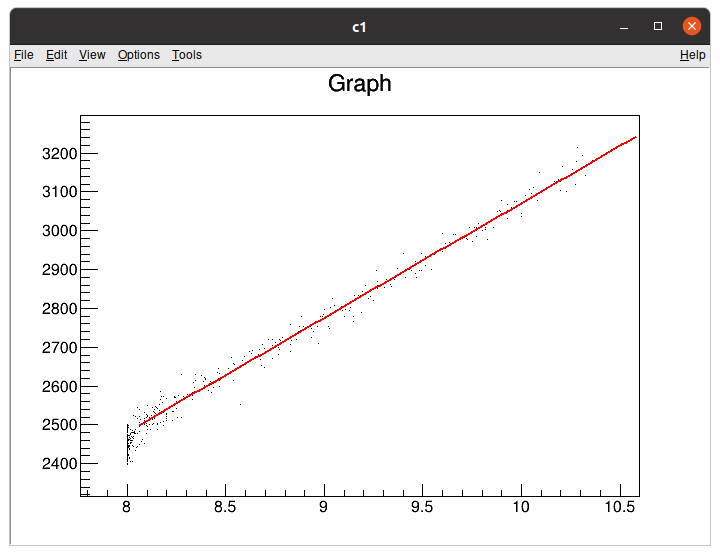
\includegraphics[width=0.5\textwidth]{9010_zt.png}
				\caption{Dependence of the~drift time on the~$z$~coordinate in 90~\%~argon and 10~\%~CO$_2$ atmosphere, fitted with a~linear function. The~fitted function gives us the~average drift velocity in the~gas and can be used for rough reconstruction in our TPC. \textcolor{red}{Swap for better image with axis labels, etc. Maybe write the~fitted equation.}}
				\label{fig:9010zt}
			\end{figure}
			
			\begin{figure}
				\centering
				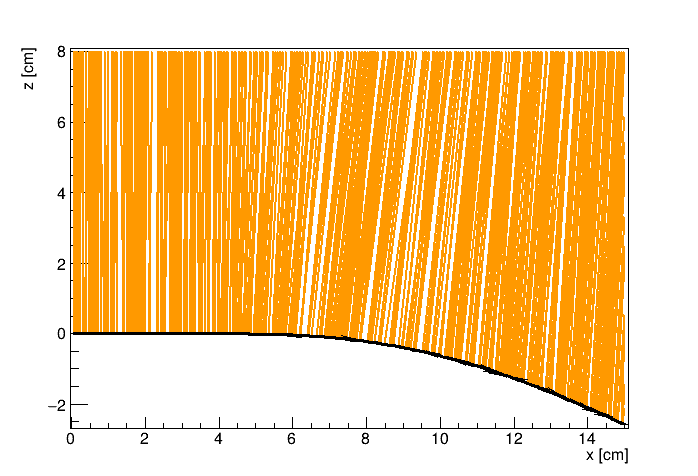
\includegraphics[width=0.5\textwidth]{9010_xz.png}
				\caption{First attempt at a~track reconstruction using only the~drift velocity. This approach works well in a~standard TPC (\textcolor{red}{ideally cite some source?}). 90~\%~argon and 10~\%~CO$_2$ atmosphere. \textcolor{red}{Swap for better image, correct coordinates.}}
				\label{fig:9010xz}
			\end{figure}
			
			\begin{figure}
				\centering
				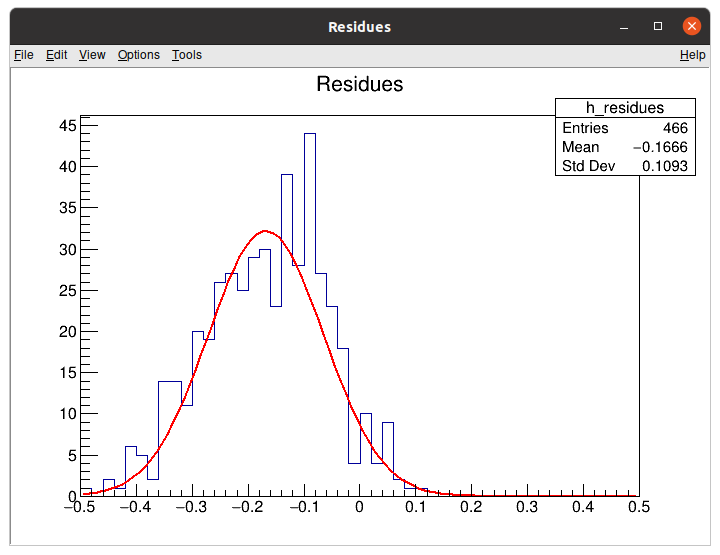
\includegraphics[width=0.5\textwidth]{9010_res.png}
				\caption{First attempt at a~track reconstruction using only the~drift velocity, residues. \textcolor{red}{Swap for better image, correct coordinates. What's causing the shift?}}
				\label{fig:9010res}
			\end{figure}
			
		\subsection{Ionization Electron Map}
		\label{sec:map}
			\textcolor{red}{Explanation of the map. Simulated on MetaCentrum, workload distribution between multiple jobs. More electrons at one location to get statistics. Two methods of reconstruction using this map. Comparison of 90/10 and 70/30 maps.}
					
			\begin{figure}
				\centering
				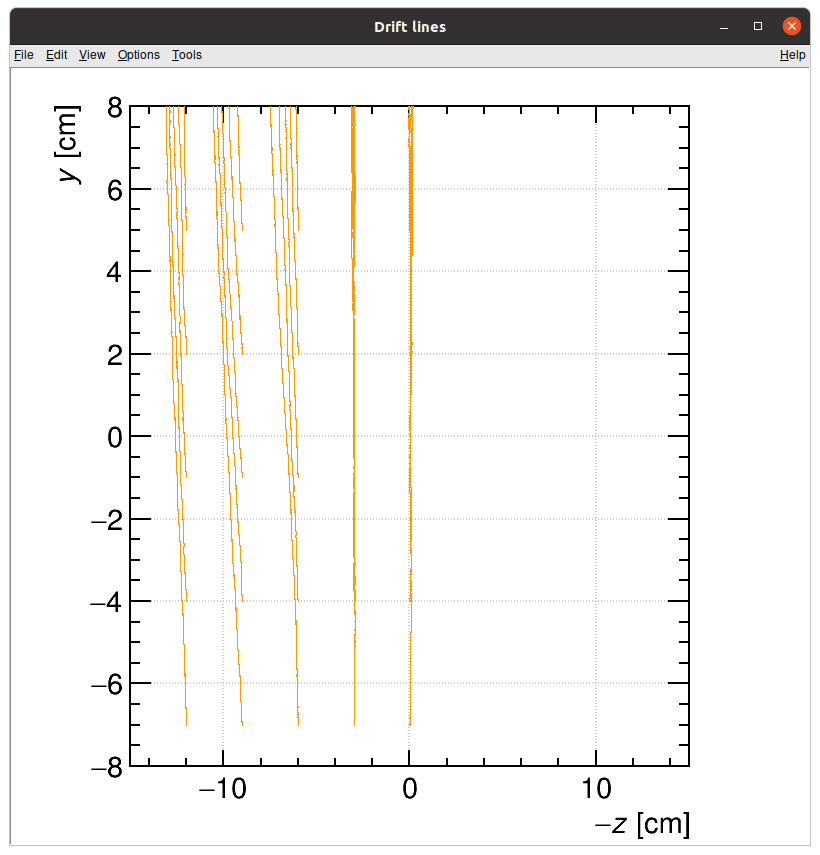
\includegraphics[width=0.5\textwidth]{map_9010_gen.png}
				\caption{Example of map generation. \textcolor{red}{Swap for better image, correct coordinates.}}
				\label{fig:map9010gen}
			\end{figure}
			
			\begin{figure}
				\centering
				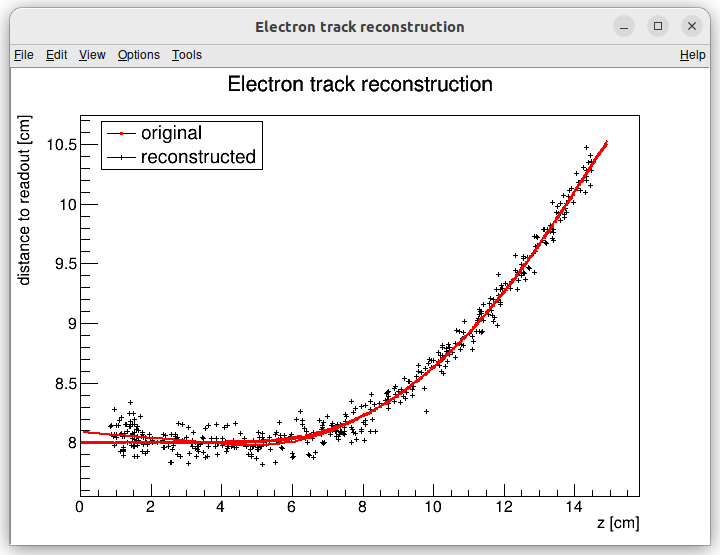
\includegraphics[width=0.5\textwidth]{9010_reco.png}
				\caption{Example reconstruction with the map. \textcolor{red}{Swap for better image, correct coordinates.}}
				\label{fig:9010reco}
			\end{figure}
			
			\subsubsection{Gradient Descent Search}
				\textcolor{red}{Gradient descent search of a point in the original space that gets mapped to the given point of the readout space (trilinear interpolation).}
			
				\paragraph{Trilinear Interpolation}
					\textcolor{red}{\newline Explanation of trilinear interpolation.}
					
			\subsubsection{Interpolating in the Inverse Grid}
				\textcolor{red}{Interpolating between known points in the readout space. Gaussian elimination, multivariate polynomial.}
				
				\begin{figure}
					\centering
					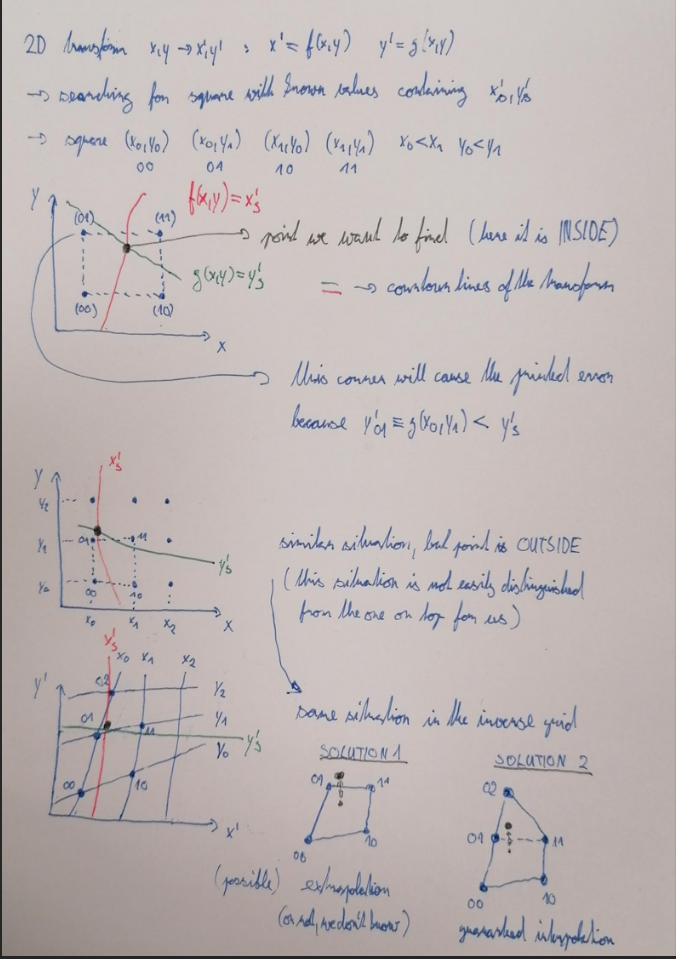
\includegraphics[width=0.8\textwidth]{interpol.png}
					\caption{Selection of the points for interpolation. \textcolor{red}{Create better images, use the explanation interpolation vs extrapolation strange property. Solution~2 probably does not make much sense.}}
					\label{fig:interpol}
				\end{figure}
		
		\subsection{Discrete Reconstruction}
			\textcolor{red}{Reconstruction with pads and time bins. Maybe testing different pads.}
			
	\section{Energy Reconstruction}
	\label{sec:energy}
		The~second stage of our reconstruction algorithm is the reconstruction of the~particle's energy using its reconstructed track (see section~\ref{sec:track}). We can achieve this by fitting the~track and extracting the~needed parameters of the~trajectory. We have tested three ways of reconstructing the~energy. Fitting is done using the~MINUIT algorithm implemented in ROOT~\cite{ROOT}. \textcolor{red}{Maybe cite some CERN article directly on MINUIT?}
		
		The~\textbf{Cubic Spline Fit} is a~rejected attempt at the~reconstruction of energy. It uses smoothly connected piecewise cubic polynomials between uniformly spaced nodes. Energy can then be computed using from the~fit parameters by computing the~radius of curvature in different points of the~fitted curve using the~known magnitude of magnetic field perpendicular to the trajectory. This approach was rejected, because tuning the fit to have reasonably stable radius of curvature is unpractical.
		
		The~\textbf{Circle and Lines Fit} was chosen as an~alternative since this corresponds to the~shape of a~trajectory of a~charged particle moving through a~finite volume with homogeneous magnetic field. The~energy of the~particle can be estimated using the~fitted radius and the~magnitude of perpendicular magnetic field in the middle of the~TPC.
		
		The~\textbf{Runge-Kutta Fit} uses the~4th order Runge-Kutta numerical integration described in section~\ref{sec:rks}. Initial~parameters of the~track (including the~particle's energy) are optimized in so that the~integrated trajectory best fits the~reconstructed one. This fit can also be performed as a~single parameter (energy) fit if we can get the initial position and orientation of the~particle on entrance to the~TPC from previous detectors (Tpx3 and MWPC, see section~\ref{sec:IEAP}).
		
		\begin{figure}
			\centering
			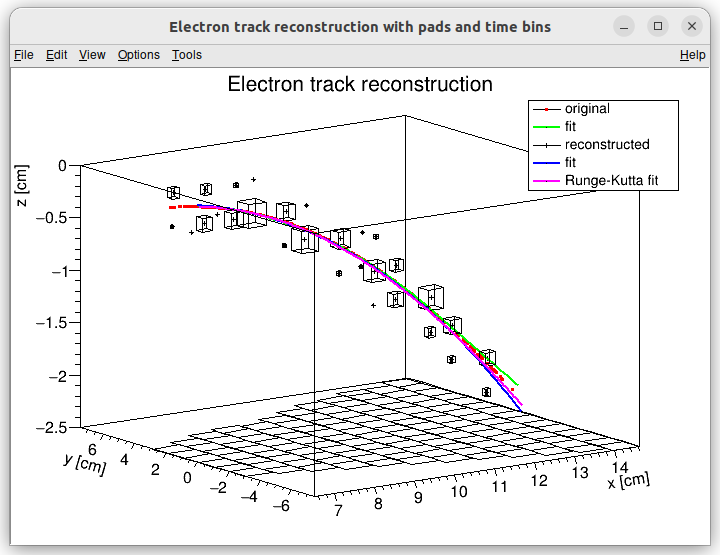
\includegraphics[width=0.5\textwidth]{9010_3d.png}
			\caption{Example of fitted reconstructed track. \textcolor{red}{Swap for better image.}}
			\label{fig:90103d}
		\end{figure}
		
		\subsection{Cubic Spline Fit}
			\textcolor{red}{Bad attempt at energy reconstruction using cubic splines.}
			
			\begin{figure}
				\centering
				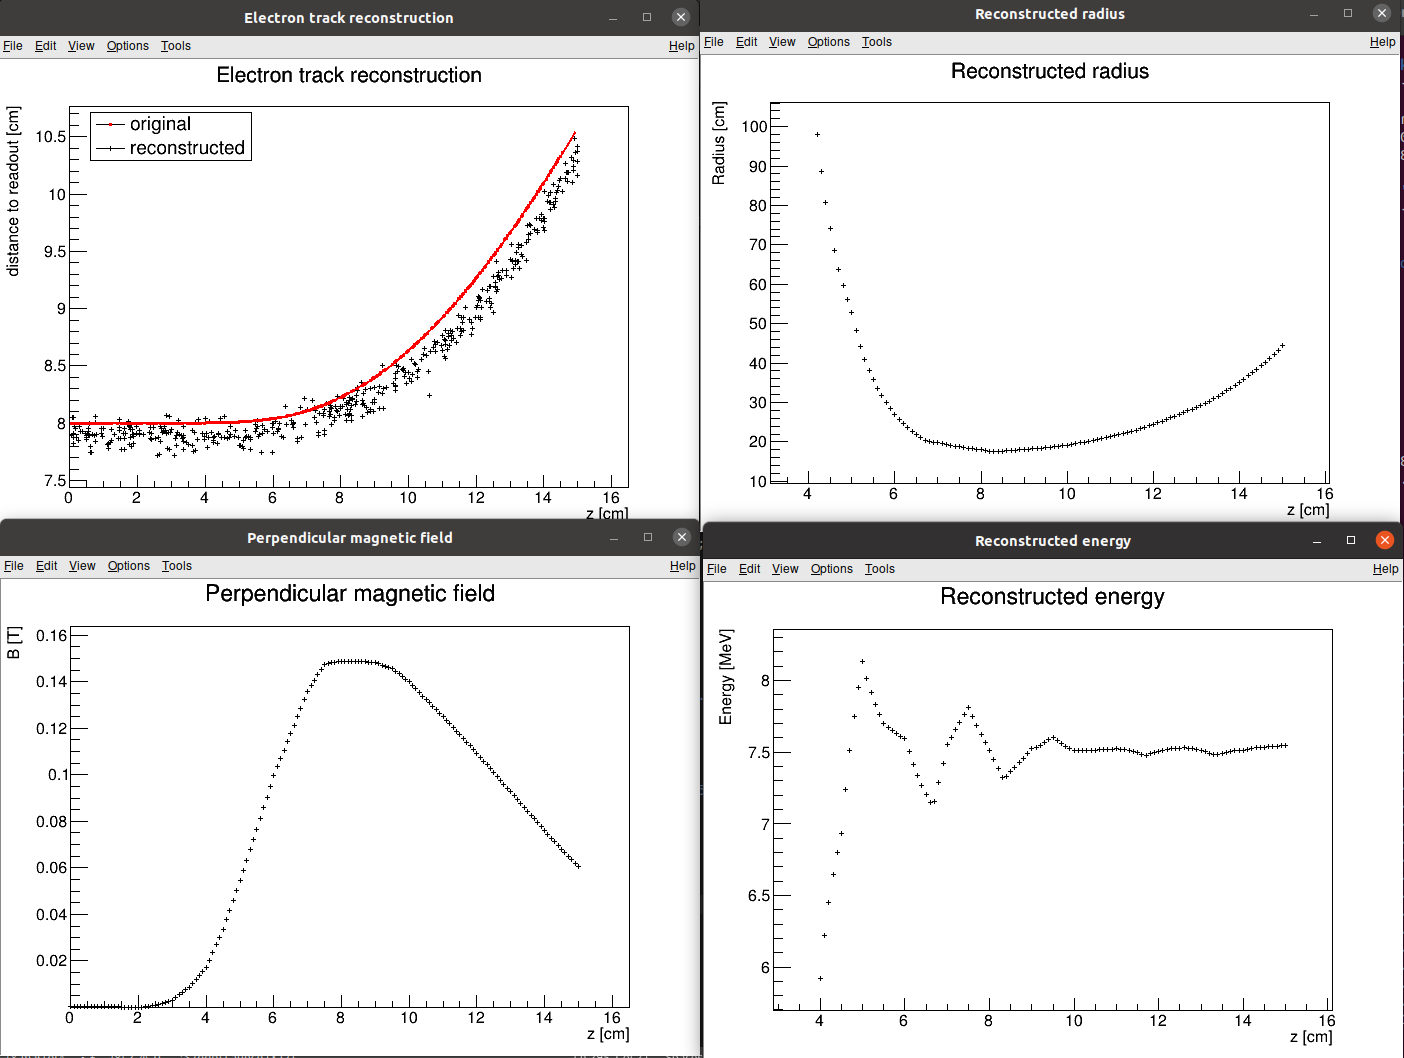
\includegraphics[width=0.8\textwidth]{9010_splines.png}
				\caption{First attempt at a~track reconstruction using only the~drift velocity. Spline energy reconstruction attempt. \textcolor{red}{Swap for better image(s) -- subfigure enviroment?, correct coordinates.}}
				\label{fig:9010splines}
			\end{figure}
		
		\subsection{Circle and Lines Fit}
			\textcolor{red}{Energy reconstruction with circle and lines fit. Trilinear interpolation of the magnetic field. Tested on Runge-Kutta sample, future testing with microscopic simulations and map simulation. Preliminary 2D version and complete 3D version. Geometry of the fit with its derivation.}
			
			\begin{figure}
				\centering
				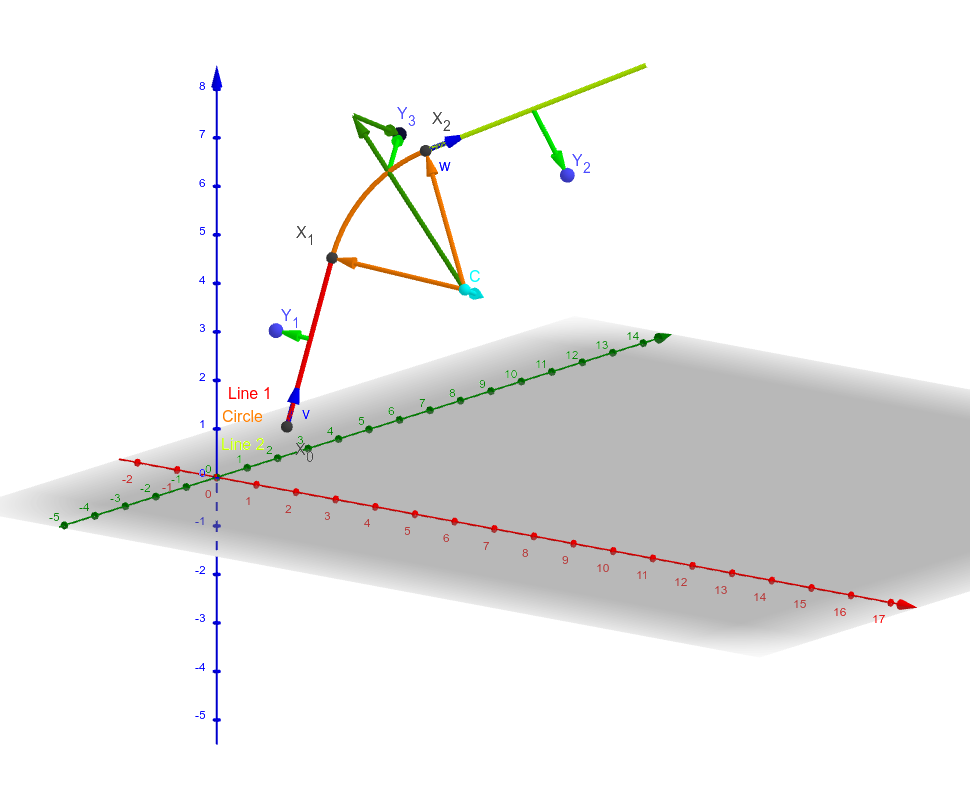
\includegraphics[width=0.8\textwidth]{circlefit.png}
				\caption{Circle and Lines Fit 3D geometry. \textcolor{red}{Swap for better image.}}
				\label{fig:circlefit}
			\end{figure}
					
			\begin{figure}
				\centering
				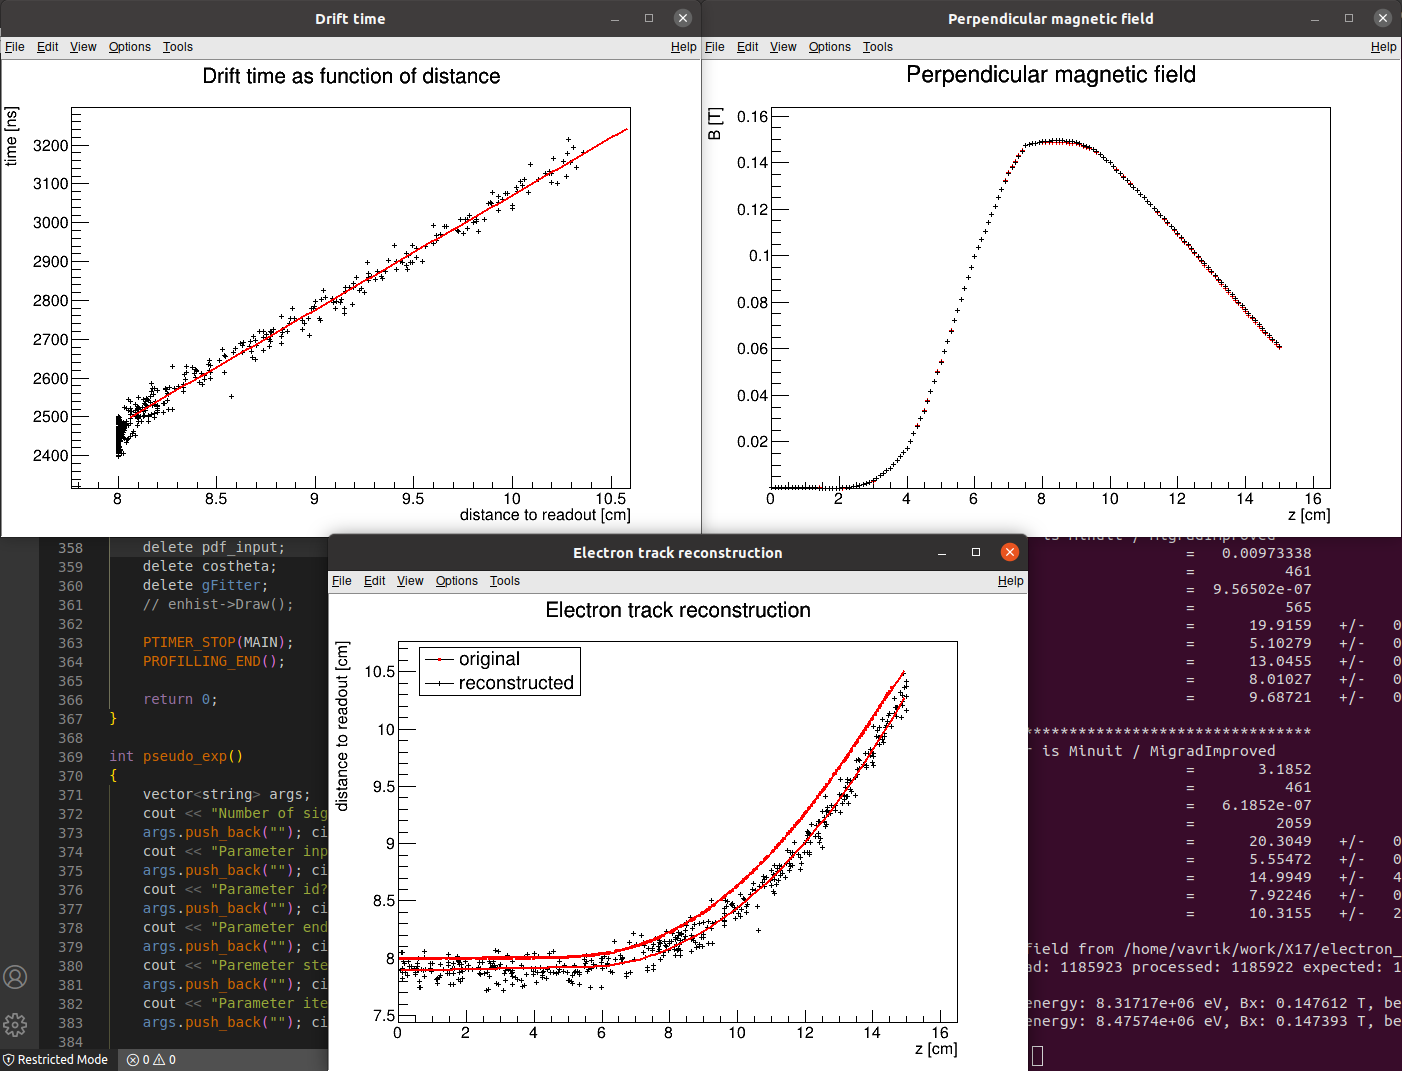
\includegraphics[width=0.8\textwidth]{9010_circle2D.png}
				\caption{First attempt at a~track reconstruction using only the~drift velocity. Circle and Lines Fit in 2D. \textcolor{red}{Swap for better image, correct coordinates.}}
				\label{fig:9010circle2D}
			\end{figure}
		
		\subsection{Runge-Kutta Fit}
			\textcolor{red}{Single parameter fit with 4th order Runge-Kutta simulated track. Future testing with microscopic simulations and map simulation. Derivation of the geometry (least squares).}
		
	\section{Conclusion}
		\textcolor{red}{Here or at the end of each section.}
		
	
	\bibliography{thesis_references}
	\bibliographystyle{unsrt}
	
\end{document}